\documentclass[]{article}
\usepackage[utf8]{inputenc}
\usepackage[T1]{fontenc}
\usepackage{graphicx}
\usepackage[portuguese]{babel}

%opening
\title{Projeto POO - Implementação do Pac-Man}
\author{11011716 - André Aranovich Florentino\\ 11003216 - Bruno Tatsuya Masunaga Santos\\ 11076916 - Lucas Eduardo Gonçalves da Rosa\\ 11006216 - Wesley Pereira da Silva}
\date{\today}

\begin{document}

\maketitle

\centerline{\textbf{Turma: A2 - Matutino}}

\section{Introdução}
Este relatório deve conter uma breve descrição do seu projeto, não podendo ultrapassar \textbf{quatro páginas}. Esta seção de introdução deve conter uma descrição sobre o projeto que escolheram implementar e seus objetivos principais. O restante do relatóri deve ser dividido na seguintes seções: Descrição das Classes, Conceitos de Orientação a Objetos Empregados, e Participação dos Integrantes do Grupo, conforme apresentado a seguir. 

\section{Descrição das classes}
Descreva de forma sucinta as principais classes implementadas e suas funções no projeto (não copie código). Além disso, construa um diagrama de classes (UML), representando seus atributos e a relação entre as classes.

\begin{itemize}
	\item Classe 1: <descrição>
	\item Classe 2: <descrição>
	\item etc...
\end{itemize}

\begin{center}
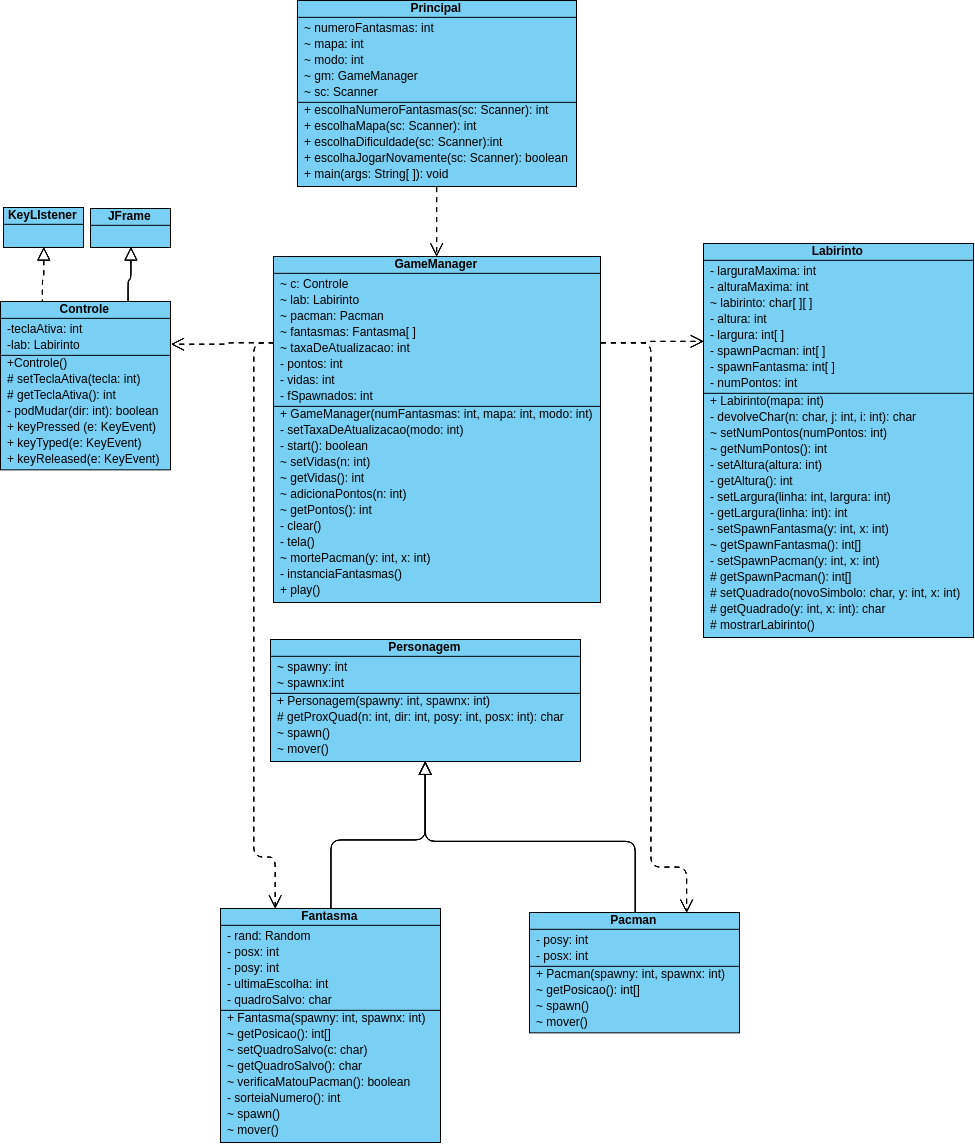
\includegraphics[width=9cm]{UML.PNG}
\end{center}

\section{Conceitos de orientação a objetos aplicados}
Descreva os conceitos de Orientação a Objetos empregados no seu projeto. Se Padrões de Projeto foram implementados, descreva quais foram e como foram usados.

\section{Participação de cada integrante do grupo}
Esta seção deve conter uma descrição da contribuição de cada integrante do grupo para realização do projeto. Por exemplo, descreva quem foi responsável pela implementação de cada classe, quem ficou responsável pela modelagem do sistema, pela confecção do relatório e geração do diagrama de classes.

\end{document}
